\section{Introduction}

This master's thesis presents a method for the computation of time bounds of integer programs.
There exist a variety of complexity analysis tools which address the same task.
These tools use different approaches for the search for time bounds.

The tool PUBS uses a non-modular approach, where a preprocessed program is analyzed at once.
This tool is discussed in the papers of Albert (\cite{pubs1}, \cite{pubs2}).

The tool CoFloCo uses an approach with cost relations, discussed in papers of Flores-Montoya (\cite{cofloco1}, \cite{cofloco2} and \cite{cofloco4}) and finally presented in his thesis \cite{cofloco3}.
This approach classifies program executions into different execution patterns called chains and performs a cost analysis yielding polynomial bounds with max and min operators. 
While this approach performs well for complex programs, it is not able to infer non-polynomial bounds.

The tool Loopus implements an amortized complexity analysis base on lexicographic ranking functions, discussed in the papers of Sinn and Zuleger (\cite{loopus1}, \cite{loopus2}).

The tool KoAT uses the computation of size bounds for inferring time bounds, discussed in the paper of Brockschmidt (\cite{koat}).
The paper presents a modular approach with ranking functions, where parts of the program can be analyzed independently and local ranking functions are lifted into a global time bounds.

The method of this master's thesis is based on the KoAT paper \cite{koat}.
It changes the methods of the KoAT paper \cite{koat} in such a way, that it is possible to infer non-monotonic bounds instead of only monotonic bounds.

To demonstrate the potentials of the presented method, the next section provides a motivating example.
Then, the second chapter introduces the preliminaries.
These include a definition of the non-monotonic bound set to represent the set of possible results of the analysis.
Furthermore, a definition of an integer program and a utility structure called a result variable graph are introduced.
Additionally, the term of a ranking function is defined and split into the terms of a time ranking function and a cost ranking function.

The third chapter introduces an operator on the non-monotonic bound set called an approximated replacement.
Non-monotonic bounds entail the difficulty, that a common substitution can yield an unsound overapproximation.
The approximated replacement is defined to solve this problem.

The fourth chapter defines the terms time, size and cost complexity, as well as time, size and cost bounds.
These definitions are more precise than definitions of the KoAT paper \cite{koat}.
The results of the new method are not representable with the definitions of the KoAT paper \cite{koat}.

The fifth and the six chapter present the new approach for the computation of time bounds and size bounds.
While the fifth chapter introduces a new theorem for the computation of time bounds, which uses a preexisting size bound, the sixth chapter introduces a new theorem for the computation of size bounds, which uses preexisting time bounds.

The seventh chapter defines two methods for the computation of cost bounds, one trivial method considering the inferred time bounds and one new method based on cost ranking functions.

The eighth chapter presents some details about the implementation of the presented method.
Then, in the ninth chapter this implementation is evaluated and compared with other tools of the same domain.

The tenth chapter concludes this thesis.
In the appendix all necessary proofs are given.

\subsection{Motivation}

We now take a look at an example to see the benefit of non-monotonic bounds.
Figure \ref{fig:motivational_example} shows a program, which takes two variables $x$ and $y$ as input and runs a loop, which decrements $x$ in each step with $t_1$ until $x$ is not greater than 0 anymore.
We can easily see, that the transition $t_1$ will be used at most $\max \braced{0, x-y}$ times.
However, since the previous method only used monotonic bounds, it only infers the bound $\abs{x}+\abs{y}$ for $t_1$.

\todo{Continue}{}

\begin{figure}
  \centering
  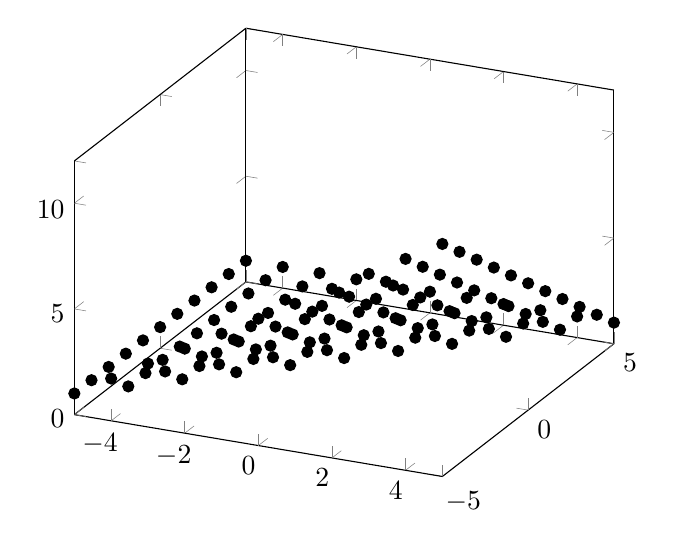
\begin{tikzpicture}
    \begin{axis}
      \addplot3 [
        unbounded coords=jump,
        mesh,
        shader=interp,
        samples at={-5,...,5},
        samples y={11},
        only marks,
      ] {1+max(x-y,0)};
    \end{axis}
  \end{tikzpicture}
  \hfil
  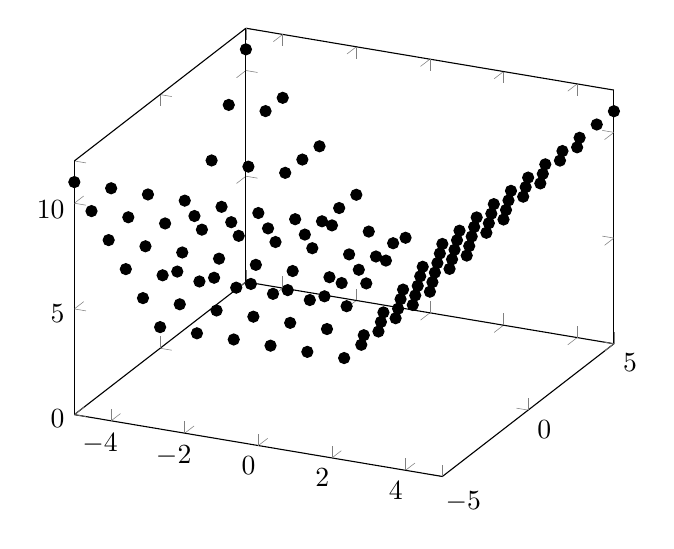
\begin{tikzpicture}
    \begin{axis}
      \addplot3 [
        unbounded coords=jump,
        mesh,
        shader=interp,
        samples at={-5,...,5},
        samples y={11},
        only marks,
      ] {1+abs(max(x,-y))+abs(max(x,-y))};
    \end{axis}
  \end{tikzpicture}
  \caption{Evaluation of the motivational example}
  \label{fig:motivational_evaluation}
\end{figure}


\begin{figure}
\centering
\begin{tikzpicture}[->,>=stealth',auto,node distance=5cm,
    thick,
    main node/.style={circle,draw,font=\sffamily\Large\bfseries},
    aligned edge/.style={align=left}]

  \node[main node] (0) {$l_0$};
  \node[main node] (1) [right of=0] {$l_1$};

  \path[every node/.style={font=\sffamily\small}]
    (0) edge[aligned edge] node {$t_0: x' = x \wedge y' = y$} (1)
    (1) edge[aligned edge, loop right] node {$t_1: x > 0 \wedge x' = x - 1 \wedge y' = -2 \cdot y$} (1)
    ;
\end{tikzpicture}
\caption{Program, where non-monotonic bounds does not yield a benefit}
\label{fig:non_beneficial_example}
\end{figure}

